\documentclass[11pt,a4paper]{article}

% ============ Idioma y codificación ============
\usepackage[utf8]{inputenc}
\usepackage[T1]{fontenc}
\usepackage[spanish]{babel}
\usepackage{textcomp}
\usepackage{microtype}

% ============ Página ============
\usepackage{geometry}
\geometry{margin=2.5cm}

% ============ Matemática, tablas, imágenes ============
\usepackage{amsmath}
\usepackage{amssymb}
\usepackage{graphicx}
\usepackage{booktabs}
\usepackage{caption}

% ============ Colores ============
\usepackage{xcolor}
\definecolor{rcblue}{RGB}{31,74,121}
\definecolor{rcgray}{RGB}{90,90,90}

% ============ Código fuente ============
\usepackage{listings}
\lstdefinestyle{pythonstyle}{
    language=Python,
    backgroundcolor=\color{gray!5},
    basicstyle=\ttfamily\footnotesize,
    keywordstyle=\color{rcblue}\bfseries,
    commentstyle=\color{gray!50!black}\itshape,
    stringstyle=\color{teal},
    numbers=left,
    numberstyle=\tiny\color{gray},
    stepnumber=1,
    numbersep=8pt,
    frame=single,
    rulecolor=\color{gray!40},
    breaklines=true,
    showstringspaces=false,
    tabsize=4,
    literate=%
        {á}{{\'a}}1 {é}{{\'e}}1 {í}{{\'i}}1 {ó}{{\'o}}1 {ú}{{\'u}}1
        {Á}{{\'A}}1 {É}{{\'E}}1 {Í}{{\'I}}1 {Ó}{{\'O}}1 {Ú}{{\'U}}1
        {ñ}{{\~n}}1 {Ñ}{{\~N}}1
}
\lstset{style=pythonstyle}

% ============ Encabezado y pie de página ============
\usepackage{fancyhdr}
\setlength{\headheight}{14pt}
\pagestyle{fancy}
\fancyhf{}
\fancyhead[L]{Redes de Computadoras}
\fancyhead[R]{Tarea 2 --- Teórico}
\fancyfoot[C]{\thepage}
\renewcommand{\headrulewidth}{0.4pt}
\renewcommand{\footrulewidth}{0.2pt}

% ============ Hipervínculos (cargar al final del preámbulo) ============
\usepackage{hyperref}
\hypersetup{
    colorlinks=true,
    linkcolor=rcblue,
    urlcolor=rcblue,
    citecolor=rcblue,
    linktoc=all,
    pdftitle={Tarea 2 - Teorico - Redes de Computadoras},
    pdfauthor={WireGuardians},
    pdfsubject={Redes de Computadoras}
}

% ============ Entornos Pregunta / Respuesta ============
\newenvironment{pregunta}{%
    \par\smallskip\noindent{\color{rcblue}\textbf{Pregunta:}}\par\smallskip\noindent
}{\par\smallskip}

\newenvironment{respuesta}{%
    \par\noindent{\color{rcgray}\textbf{Respuesta:}}\par\smallskip\noindent
}{\par\bigskip}

% ============ Encabezados de sección/ejercicio con entrada al índice ============
\setcounter{tocdepth}{2}
\newcommand{\seccionprincipal}[1]{%
    \section*{#1}\addcontentsline{toc}{section}{#1}
}
\newcommand{\subseccion}[1]{%
    \subsection*{#1}\addcontentsline{toc}{subsection}{#1}
}

\begin{document}

% ==================== CARÁTULA ====================
\begin{titlepage}
    \thispagestyle{empty}
    \centering
    \vspace*{1cm}
    {\large Universidad Nacional de Córdoba\par}
    {\large Facultad de Ciencias Exactas, Físicas y Naturales\par}
    {\large Ingeniería en Computación\par}

    \vspace{1cm}
    \rule{\linewidth}{0.4pt}
    \vspace{1.5cm}

    {\Large Redes de Computadoras\par}
    \vspace{0.4cm}
    {\huge\bfseries Tarea 2 --- Teórico\par}
    \vspace{0.4cm}
    {\large Sobre el Capítulo 3: Transmisión de Datos\par}

    \vspace{1.5cm}
    \rule{\linewidth}{0.4pt}
    \vspace{2cm}

    {\Large Grupo WireGuardians\par}
    \vspace{1cm}

    \begin{tabular}{lll}
        \toprule
        \textbf{Integrante} & \textbf{DNI} & \textbf{Mail UNC} \\
        \midrule
        Viberti, Benjamin & 46224179 & \texttt{b.viberti@mi.unc.edu.ar} \\
        Espinoza Sutta, Aaron Alejandro & 96009173 & \texttt{aaron.espinoza\_4500@mi.unc.edu.ar} \\
        Cleri, Juan Ignacio & 46452662 & \texttt{ignacio.cleri@mi.unc.edu.ar} \\
        Pineda, Juan Ignacio & 45591343 & \texttt{juan.ignacio.pineda@mi.unc.edu.ar} \\
        Grafión, Atilio Leonel & 43940195 & \texttt{atilio.grafion@mi.unc.edu.ar} \\
        Badenes, Tomas & 44785038 & \texttt{tomasbadenes@mi.unc.edu.ar} \\
        Oviedo, Ignacio Nicolas & 43940195 & \texttt{ignacio.oviedo.239@mi.unc.edu.ar} \\
        Mendez, Jorge Nicolas & 41301342 & \texttt{jorge.mendez@mi.unc.edu.ar} \\
        \bottomrule
    \end{tabular}

    \vfill
    {\large 2\textsuperscript{do} Cuatrimestre 2026\par}
\end{titlepage}

% ==================== ÍNDICE ====================
\pagenumbering{roman}
\tableofcontents
\newpage

\pagenumbering{arabic}
\setcounter{page}{1}

% ==================== b) PREGUNTAS DE REPASO ====================
\seccionprincipal{b) Preguntas de repaso}

\subseccion{3.1. ¿En qué se diferencia un medio guiado de un medio no guiado?}

\begin{respuesta}
En ambos tipos de medios la comunicación se realiza mediante ondas electromagnéticas; la diferencia radica en \textbf{cómo se propaga la onda}:

\begin{itemize}
    \item \textbf{Medio guiado:} La onda se transmite confinada a lo largo de un camino físico. Ejemplos: par trenzado, cable coaxial, fibra óptica.
    \item \textbf{Medio no guiado (inalámbrico):} La onda se propaga libremente, sin estar confinada a un camino físico. Ejemplos: propagación a través del aire, el mar o el vacío.
\end{itemize}
\end{respuesta}

\subseccion{3.2. ¿Cuáles son las diferencias entre una señal electromagnética analógica y una digital?}

\begin{respuesta}
Toda señal electromagnética, considerada como función del tiempo, puede ser tanto analógica como digital. La diferencia entre ambas está en cómo varía la intensidad de la señal en el tiempo:

\begin{itemize}
    \item \textbf{Señal analógica:} Es una onda electromagnética que varía continuamente en el tiempo, sin saltos ni discontinuidades, y puede tomar cualquier valor dentro de un rango continuo. Según su espectro, puede propagarse tanto por medios guiados (par trenzado, cable coaxial, fibra óptica) como no guiados (atmósfera, espacio).
    \item \textbf{Señal digital:} Es una secuencia de pulsos de tensión que se mantiene constante durante un intervalo de tiempo, tras el cual cambia abruptamente a otro valor constante. Por ejemplo, un nivel de tensión positiva puede representar un bit 0 y un nivel de tensión negativa un bit 1.
\end{itemize}

\textbf{Ventajas y desventajas de la señalización digital frente a la analógica:}
\begin{itemize}
    \item \textit{Ventaja:} en términos generales es más económica y menos susceptible a las interferencias de ruido.
    \item \textit{Desventaja:} las señales digitales sufren más con la atenuación que las señales analógicas.
\end{itemize}
\end{respuesta}

\subseccion{3.3. ¿Cuáles son las tres características más importantes de una señal periódica?}

\begin{respuesta}
Una señal periódica se caracteriza por contener un patrón que se repite a lo largo del tiempo. Matemáticamente, una señal $s(t)$ es periódica si y solo si:

\[
s(t + T) = s(t), \quad -\infty < t < \infty
\]

donde $T$ es el período de la señal (el menor valor que verifica la ecuación).

Las \textbf{tres características más importantes} que definen a una señal periódica son:

\begin{itemize}
    \item \textbf{Amplitud (A):} El valor máximo que alcanza la señal en el tiempo (amplitud de pico), normalmente medido en voltios.
    \item \textbf{Frecuencia (f):} La razón, en ciclos por segundo o Hercios (Hz), a la que la señal se repite. Su parámetro equivalente es el período (T), definido como el tiempo transcurrido entre dos repeticiones consecutivas, cumpliéndose que $T = 1/f$.
    \item \textbf{Fase ($\varphi$):} Una medida de la posición relativa de la señal dentro de un período de la misma.
\end{itemize}
\end{respuesta}

\subseccion{3.4. ¿Cuántos radianes hay en $360^\circ$?}

\begin{respuesta}
El radián es la unidad de medida angular basada en la relación entre el arco y el radio de una circunferencia: un ángulo de 1 radián es aquel que subtiende un arco de longitud igual al radio.

Dado que el perímetro completo de una circunferencia equivale a $2\pi$ veces su radio, una vuelta completa ($360^\circ$) equivale a $2\pi$ radianes:

\[
360^\circ = 2\pi \text{ radianes}
\]
\end{respuesta}

\subseccion{3.5. ¿Cuál es la relación entre la longitud de onda y la frecuencia en una onda seno?}

\begin{respuesta}
La longitud de onda ($\lambda$) se define como la distancia que ocupa un ciclo de la señal, o equivalentemente, la distancia entre dos puntos de igual fase en dos ciclos consecutivos. Representa la contraparte espacial del período (T), que es su equivalente en el dominio temporal.

Si la señal se propaga a una velocidad $v$, la longitud de onda se relaciona con el período mediante:

\[
\lambda = v \cdot T
\]

Dado que $T = 1/f$, esta expresión es equivalente a:

\[
\lambda \cdot f = v
\]

Es decir, \textbf{la longitud de onda y la frecuencia son inversamente proporcionales}: a mayor frecuencia, menor longitud de onda, y viceversa, para una misma velocidad de propagación $v$.
\end{respuesta}

\subseccion{3.6. ¿Cuál es la relación entre el espectro de una señal y su ancho de banda?}

\begin{respuesta}
Según el análisis de Fourier, cualquier señal electromagnética puede descomponerse en una colección de componentes sinusoidales (ondas seno), cada una con su propia amplitud, frecuencia y fase. Mientras la señal $s(t)$ describe su comportamiento en el dominio del tiempo, la función $S(f)$ la describe en el dominio de la frecuencia, especificando las amplitudes de sus componentes.

A partir de esto:
\begin{itemize}
    \item \textbf{Espectro:} Es el conjunto de frecuencias que constituyen una señal.
    \item \textbf{Ancho de banda absoluto:} Es la anchura de ese espectro, es decir, la diferencia entre su frecuencia más alta y más baja.
\end{itemize}

En la práctica, muchas señales (por ejemplo, cualquier onda digital) tienen un espectro y, por lo tanto, un ancho de banda absoluto infinito. Sin embargo, la mayor parte de su energía se concentra en una banda de frecuencias relativamente estrecha; a esa banda se la denomina \textbf{ancho de banda efectivo} (o simplemente ancho de banda).

\textbf{Relación con la transmisión real:} Ningún sistema de transmisión puede portar un ancho de banda infinito, y cuanto mayor es el ancho de banda transmitido, mayor es el costo. Por eso, en la práctica se transmite una versión de ancho de banda limitado de la señal original. Esta limitación introduce distorsión: cuanto más se restringe el ancho de banda respecto del espectro original, mayor es la distorsión y mayor la probabilidad de errores en el receptor.
\end{respuesta}

\subseccion{3.7. ¿Qué es la atenuación?}

\begin{respuesta}
La atenuación es la pérdida de energía que sufre una señal a medida que se propaga a través de un medio de transmisión, decayendo con la distancia recorrida. Es una de las dificultades fundamentales de la transmisión, junto con la distorsión de retardo y el ruido, y provoca que la señal recibida difiera de la señal originalmente transmitida (degradando su calidad en señales analógicas, o generando bits erróneos en señales digitales).

\textbf{Comportamiento según el tipo de medio:}
\begin{itemize}
    \item \textbf{Medios guiados:} La atenuación suele ser exponencial, por lo que se expresa como un valor constante en decibelios por unidad de longitud.
    \item \textbf{Medios no guiados:} La atenuación es una función más compleja de la distancia, dependiente además de las condiciones atmosféricas.
\end{itemize}

\textbf{Consideraciones respecto a la atenuación:}
\begin{enumerate}
    \item La señal recibida debe tener suficiente energía para que el receptor pueda detectarla adecuadamente.
    \item Debe conservar un nivel notoriamente mayor que el del ruido para poder recibirse sin error.
    \item La atenuación es, habitualmente, una función creciente de la frecuencia (afecta más a las frecuencias altas).
\end{enumerate}

\textbf{Mitigación:} Los dos primeros problemas se resuelven controlando la energía de la señal mediante amplificadores o repetidores, ubicados a distancias adecuadas cuando la atenuación acumulada se vuelve inaceptable. El tercer problema se aborda con técnicas de ecualización de la atenuación en una banda de frecuencias dada.
\end{respuesta}

\subseccion{3.8. Defina la capacidad de un canal}

\begin{respuesta}
Se denomina \textbf{capacidad del canal} a la velocidad máxima a la que se pueden transmitir datos en un canal (o ruta de comunicación de datos) bajo unas condiciones dadas. Para el caso de datos digitales, la pregunta que responde es en qué medida los efectos nocivos que distorsionan o corrompen la señal limitan la velocidad de transmisión.
\end{respuesta}

\subseccion{3.9. ¿Qué factores clave afectan a la capacidad de un canal?}

\begin{respuesta}
Hay \textbf{cuatro conceptos relacionados entre sí} que determinan la capacidad de un canal:
\begin{itemize}
    \item \textbf{La velocidad de transmisión de los datos:} Velocidad, expresada en bits por segundo (bps), a la que se pueden transmitir los datos.
    \item \textbf{El ancho de banda:} Ancho de banda de la señal transmitida, limitado por el transmisor y por la naturaleza del medio; se mide en hercios.
    \item \textbf{El ruido:} Nivel medio de ruido presente en el camino de transmisión.
    \item \textbf{La tasa de errores:} Tasa a la que ocurren errores (recibir un 1 habiendo transmitido un 0, o viceversa).
\end{itemize}

\textbf{Relación entre estos factores:}
\begin{itemize}
    \item \textbf{Ancho de banda de Nyquist} (canal sin ruido): dado un ancho de banda $B$, la máxima velocidad de señal alcanzable es $2B$. Para señales con $M$ niveles discretos, la capacidad es $C = 2B \log_2 M$.
    \item \textbf{Capacidad de Shannon} (canal con ruido): relaciona la capacidad con el ancho de banda y la relación señal-ruido (SNR):
    \[
    C = B \log_2(1 + SNR)
    \]
\end{itemize}

Esta fórmula representa el límite teórico máximo: dado un ancho de banda y un nivel de ruido, mayor SNR permite mayor capacidad. En la práctica se obtienen velocidades menores, ya que la fórmula supone únicamente ruido térmico y no contempla otros efectos como el ruido impulsivo o las distorsiones de atenuación y retardo.
\end{respuesta}

% ==================== c) EJERCICIOS ====================
\seccionprincipal{c) Ejercicios (3.1 a 3.20)}

\subseccion{Ejercicio 3.1}

\subsubsection*{a)}
\begin{pregunta}
En una configuración multipunto, sólo un dispositivo puede trasmitir cada vez, ¿por qué?
\end{pregunta}
\begin{respuesta}
En este caso depende exactamente de cómo esté implementado el medio de transmisión: si este cuenta con más de un canal de transmisión de datos (usando Multiplexación por División de Frecuencias), pero en un caso básico con un único canal, sí se puede decir que solo se puede transmitir un dispositivo a la vez.
\end{respuesta}

\subsubsection*{b)}
\begin{pregunta}
Hay dos posibles aproximaciones que refuerzan la idea de que, en un momento dado, sólo un dispositivo puede transmitir. En un sistema centralizado, una estación es la responsable del control y podrá transmitir o decidir que lo haga cualquier otra. En el método descentralizado, las estaciones cooperan entre sí, estableciéndose una serie de turnos. ¿Qué ventajas y desventajas presentan ambas aproximaciones?
\end{pregunta}
\begin{respuesta}
\paragraph*{Caso 1: Sistema Centralizado.}
\textbf{Ventajas:} Es más sencillo evitar transmisiones a la vez ya que el que daría la orden directamente sería la estación de control; también, al evitar el sistema de turnos, en teoría se puede optimizar el uso del medio de transmisión.

\textbf{Desventajas:} Todo el control depende de una única estación, la cual puede quedar fuera de servicio y parar en seco las transmisiones de todas las demás estaciones.

\paragraph*{Caso 2: Sistema Descentralizado.}
\textbf{Ventajas:} Puede seguir funcionando incluso si una o varias estaciones están fuera de servicio.

\textbf{Desventajas:} El sistema es menos óptimo, ya que puede que el canal sea necesitado por alguna estación pero no se use porque no es su turno.
\end{respuesta}

\subseccion{Ejercicio 3.2}
\begin{pregunta}
Una señal tiene una frecuencia fundamental de 1000 Hz. ¿Cuál es su período?
\end{pregunta}
\begin{respuesta}
Si una señal tiene una frecuencia fundamental $f=1000\text{Hz} \rightarrow T=\dfrac{1}{f}=\dfrac{1}{1000\text{Hz}}= 1\text{ms}$
\end{respuesta}

\subseccion{Ejercicio 3.3}
\begin{pregunta}
Simplifique las siguientes expresiones:

a) $\sin(2\pi ft - \pi) + \sin(2\pi ft + \pi)$

b) $\sin(2\pi f t) + \sin(2\pi f t - \pi)$
\end{pregunta}
\begin{respuesta}
\textbf{a)}
\[
\sin(2\pi ft - \pi) + \sin(2\pi ft + \pi) = -\sin(2\pi ft) + \left(-\sin(2\pi ft)\right) = -2\sin(2\pi ft)
\]

\textbf{b)}
\[
\sin(2\pi f t) + \sin(2\pi f t - \pi) = \sin(2\pi f t) + (-\sin(2\pi f t)) = 0
\]
\end{respuesta}

\subseccion{Ejercicio 3.4}
\begin{pregunta}
El sonido se puede modelar mediante funciones sinusoidales. Compare la frecuencia relativa y la longitud de onda de las notas musicales. Piense que la velocidad del sonido es igual a 330 m/s y que las frecuencias de una escala musical son:
\end{pregunta}
\begin{respuesta}
Sea $v$ la velocidad del sonido, $\lambda$ la longitud de onda y $f$ la frecuencia de la nota:

\[
\lambda = \frac{v}{f}
\]

\begin{center}
\begin{tabular}{lcccccccc}
    \toprule
    Nota & DO & RE & MI & FA & SOL & LA & SI & DO \\
    \midrule
    $f$ (Hz) & 264 & 297 & 330 & 352 & 396 & 440 & 495 & 528 \\
    $\lambda$ (m) & 1.2500 & 1.1111 & 1.0000 & 0.9375 & 0.8333 & 0.7500 & 0.6667 & 0.6250 \\
    \bottomrule
\end{tabular}
\end{center}

Podemos ver cómo a mayor frecuencia de la nota, menor es la longitud de onda.
\end{respuesta}

\subseccion{Ejercicio 3.5}
\begin{pregunta}
Si la curva trazada con una línea continua de la Figura 3.17 representa a $\sin(2nt)$, ¿qué función corresponde a la línea discontinua? En otras palabras, la línea discontinua se puede expresar como $A\sin(2nft+\phi)$, ¿qué son $A$, $f$ y $\phi$?

\begin{center}
    
\includegraphics[width=0.6\linewidth,height=0.35\textheight,keepaspectratio]{imagenes/image.png}
\end{center}
\end{pregunta}
\begin{respuesta}
La línea discontinua corresponde a una función seno a la cual se le cambió la frecuencia $f$ (esta pasó a ser el doble de la anterior), se le aplicó un desfasaje $\phi$ (de más o menos $0.5$) y además se le aumentó la amplitud $A$ (una amplitud mayor a 1).
\end{respuesta}

\subseccion{Ejercicio 3.6}
\begin{pregunta}
Exprese la señal \textit{(1 + 0,1 $\cos 5t$) $\cos 100t$} como combinación lineal de funciones sinusoidales; encuentre la amplitud, frecuencia y fase de cada una de las componentes. (Sugerencia: use la expresión del $\cos a \cos b$).
\end{pregunta}
\begin{respuesta}
Distribuimos el producto:
\[
s(t) = (1)(\cos100t) + (0{,}1\cos5t)(\cos100t) = \cos100t + 0{,}1\cos5t\cos100t
\]

Aplicamos la identidad trigonométrica que sugiere la consigna en el segundo término: $\cos a\cos b=\tfrac12[\cos(a-b)+\cos(a+b)]$

\[
0{,}1\cos100t\cos5t = 0{,}1\cdot\frac12\big[\cos(100t-5t)+\cos(100t+5t)\big] = 0{,}1\cdot\frac12\big[\cos95t+\cos105t\big] = 0{,}05\cos95t+0{,}05\cos105t
\]

\[
s(t) = \cos100t + 0{,}05\cos95t + 0{,}05\cos105t
\]

\begin{center}
\begin{tabular}{lcccc}
    \toprule
    Término & Amplitud & $\omega$ (rad/s) & $f=\omega/2\pi$ (Hz) & Fase \\
    \midrule
    $\cos100t$ & 1 & 100 & $\approx 15{,}92$ & 0 \\
    $0{,}05\cos95t$ & 0,05 & 95 & $\approx 15{,}12$ & 0 \\
    $0{,}05\cos105t$ & 0,05 & 105 & $\approx 16{,}71$ & 0 \\
    \bottomrule
\end{tabular}
\end{center}
\end{respuesta}

\subseccion{Ejercicio 3.7}
\begin{pregunta}
Encuentre el período de la función $f(t)=(10\cos t)^2$.
\end{pregunta}
\begin{respuesta}
\[
f(t) = (10\cos t)^2 = 100\cos^2t
\]

Usamos la identidad de ángulo doble $\cos^2t = \dfrac{1+\cos2t}{2}$:

\[
f(t) = 100\cdot\frac{1+\cos2t}{2}= 50 + 50\cos2t
\]

La frecuencia angular es $\omega=2$ rad/s, y el período es $T=2\pi/\omega$:

\[
T = \frac{2\pi}{2} = \pi
\]
\end{respuesta}

\subseccion{Ejercicio 3.9}
\begin{pregunta}
La Figura 3.4 muestra el efecto resultante al eliminar las componentes de alta frecuencia de un pulso cuadrado, considerando sólo las componentes de baja frecuencia. ¿Cómo sería la señal resultante en el caso contrario (es decir, quedándose con todos los armónicos de frecuencia alta y eliminando los de bajas frecuencias)?

\begin{center}
    
\includegraphics[width=0.6\linewidth,height=0.35\textheight,keepaspectratio]{imagenes/image-1.png}
\end{center}
\end{pregunta}
\begin{respuesta}
La señal resultante, quedándose con todos los armónicos de frecuencias altas y eliminando los de bajas frecuencias, pierde todo lo \textit{plano} de la onda cuadrada. Lo que sobrevive son unos picos angostos justo donde antes había un salto brusco (los flancos).
\end{respuesta}

\subseccion{Ejercicio 3.10}
\begin{pregunta}
La Figura 3.5b muestra la función correspondiente a un pulso rectangular en el dominio de la frecuencia. Este pulso puede corresponder a un 1 digital en un sistema de comunicación. Obsérvese que se necesita un número infinito de frecuencias (con amplitud decreciente cuanto mayor es la frecuencia). ¿Qué implicaciones tiene este hecho en un sistema de transmisión real?

\begin{center}
    
\includegraphics[width=0.6\linewidth,height=0.35\textheight,keepaspectratio]{imagenes/image-2.png}
\end{center}
\end{pregunta}
\begin{respuesta}
Las implicaciones que tiene este hecho en un sistema real son: como ningún canal de transmisión tiene ancho de banda infinito, en algún punto se pierden las componentes de frecuencia más alta del pulso, que son justamente las que le dan sus bordes filosos. Como consecuencia, el pulso que llega al receptor ya no conserva la forma rectangular ideal, sino que aparece con los flancos redondeados y estirado en el tiempo. Cuanto menor sea el ancho de banda disponible, mayor es esa distorsión.
\end{respuesta}

% ==================== d) MODULACIÓN AM ====================
\seccionprincipal{d) Modulación en AM en Python}

Para este punto se implementó el código de graficación de la modulación AM que aparece en el blog indicado en la consigna (el cual también incluye un segundo script que reproduce las mismas señales como audio, pero no se usó porque no se ajusta al objetivo de \textit{ver} el efecto de cada parámetro). El código, tal como se implementó, es el siguiente:

\lstinputlisting[style=pythonstyle,caption={\texttt{modulacion\_am.py}}]{modulacion_am.py}

El código grafica tres señales: la moduladora (la que contiene la información), la portadora (de mayor frecuencia) y el resultado de modularlas en amplitud. La señal AM se calcula como $A_p \cdot (1 + k_a \cos(2\pi f_m t)) \cdot \cos(2\pi f_p t)$: el término entre paréntesis es la envolvente, y $k_a$ controla cuánto varía esa envolvente respecto a la portadora.

Al correr el código con distintos parámetros notamos que la ventana de tiempo original (de 0 a 1 segundo, con solo 1000 muestras) no alcanza a representar bien portadoras de decenas de miles de Hz: para que se vean correctamente sus oscilaciones hace falta muestrear muchas más veces por segundo. Por eso, para las pruebas que siguen ajustamos la ventana de tiempo y la cantidad de muestras según la frecuencia usada en cada caso (sin tocar las fórmulas del código original), de forma de poder ver con claridad unos pocos ciclos de la envolvente con la portadora bien resuelta dentro de cada uno.

Como caso de referencia partimos de $A_p=5$, $f_p=40000$ Hz, $A_m=5$, $f_m=4000$ Hz y $k_a=1$ (el valor de $k_a$ que da la modulación \textit{ideal}, en la que la envolvente llega justo a cero en sus mínimos sin cruzarlo):

\begin{figure}[h!]
    \centering
    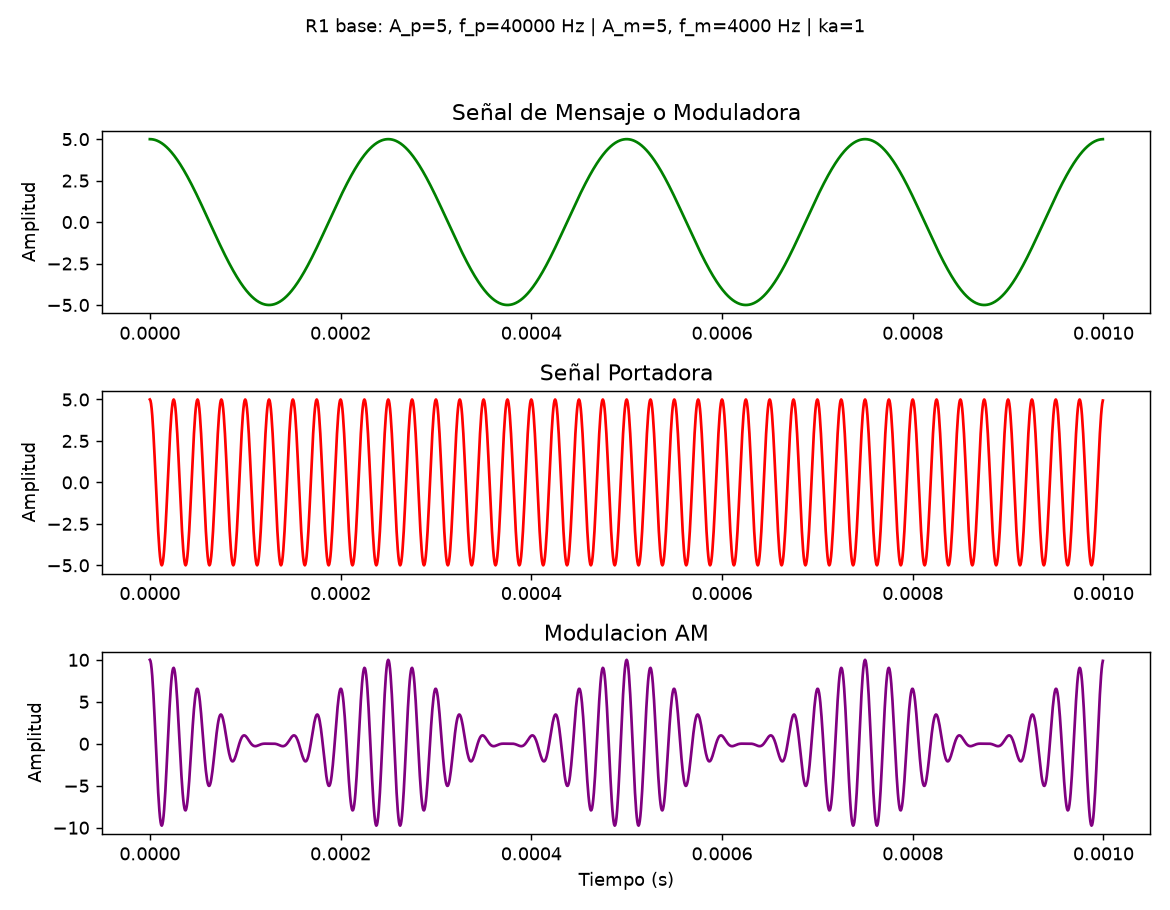
\includegraphics[width=0.75\linewidth]{imagenes/am-r1-base.png}
    \caption{Corrida base: $A_p=5$, $f_p=40000$ Hz, $A_m=5$, $f_m=4000$ Hz, $k_a=1$}
\end{figure}

Se distinguen los 40 ciclos de portadora que corresponden a 40000 Hz durante 1 ms, y los 4 ciclos de moduladora que corresponden a 4000 Hz en esa misma ventana. La envolvente de la señal AM sigue exactamente la forma de la moduladora, tocando el cero en cada mínimo.

\subsection*{Variando la portadora}

Primero probamos subir la amplitud de la portadora a 10, manteniendo todo lo demás igual:

\begin{figure}[h!]
    \centering
    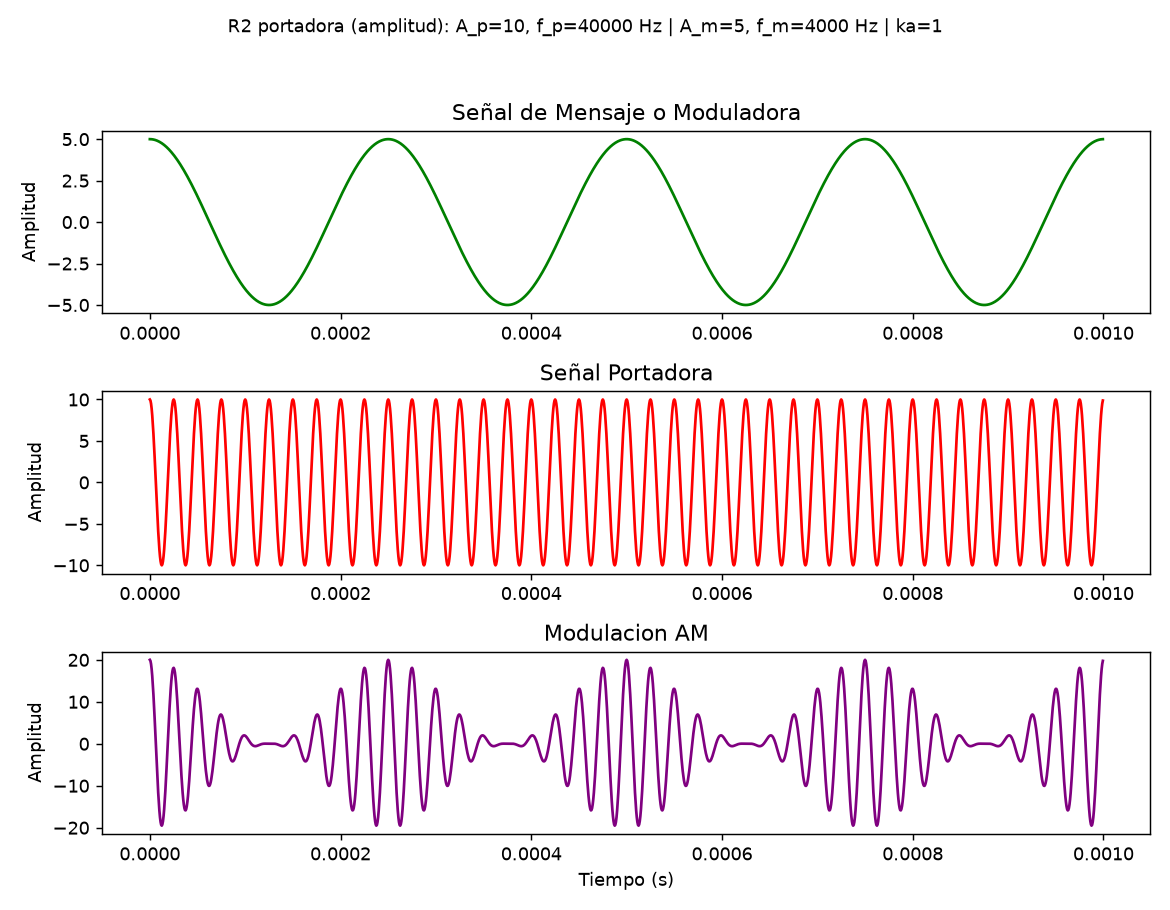
\includegraphics[width=0.75\linewidth]{imagenes/am-r2-portadora-amplitud.png}
    \caption{Portadora con mayor amplitud: $A_p=10$}
\end{figure}

El resultado tiene exactamente la misma forma que la corrida base, pero escalada al doble: tanto la portadora como la señal AM llegan ahora al doble de su valor anterior. Tiene sentido, porque $A_p$ multiplica a toda la expresión de la señal AM, así que cambiarla solo estira o achica verticalmente el gráfico sin modificar la forma de la envolvente.

Después bajamos la frecuencia de la portadora a 20000 Hz:

\begin{figure}[h!]
    \centering
    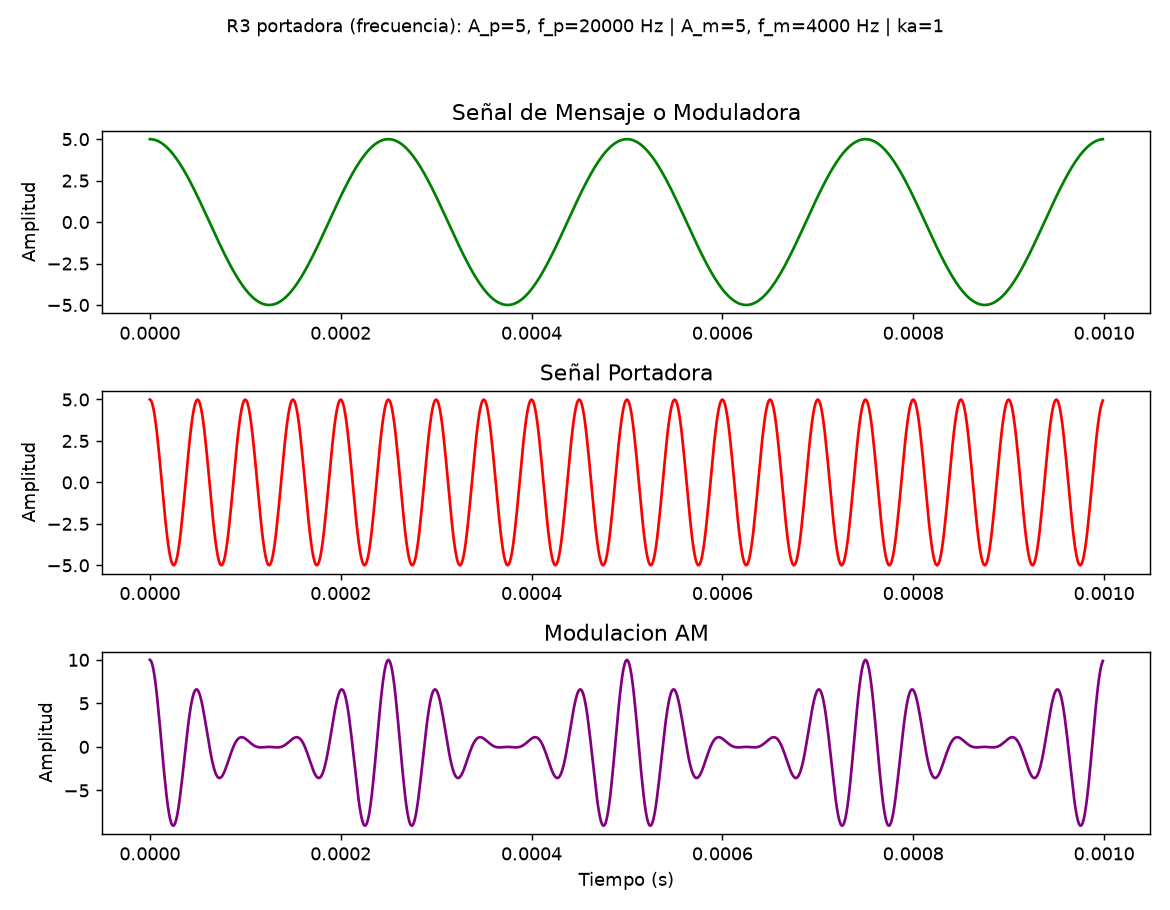
\includegraphics[width=0.75\linewidth]{imagenes/am-r3-portadora-frecuencia.png}
    \caption{Portadora con menor frecuencia: $f_p=20000$ Hz}
\end{figure}

Acá sí cambia algo relevante: en la misma ventana de 1 ms ahora entran 20 ciclos de portadora en lugar de 40, es decir la mitad. La envolvente, que depende de la moduladora y no de la portadora, se mantiene igual. Esto confirma que $f_p$ solo determina qué tan rápido oscila la portadora dentro de cada lóbulo de la envolvente, sin afectar la forma de esa envolvente.

\subsection*{Variando la moduladora}

Con la portadora en sus valores originales, bajamos la amplitud de la moduladora a 1:

\begin{figure}[h!]
    \centering
    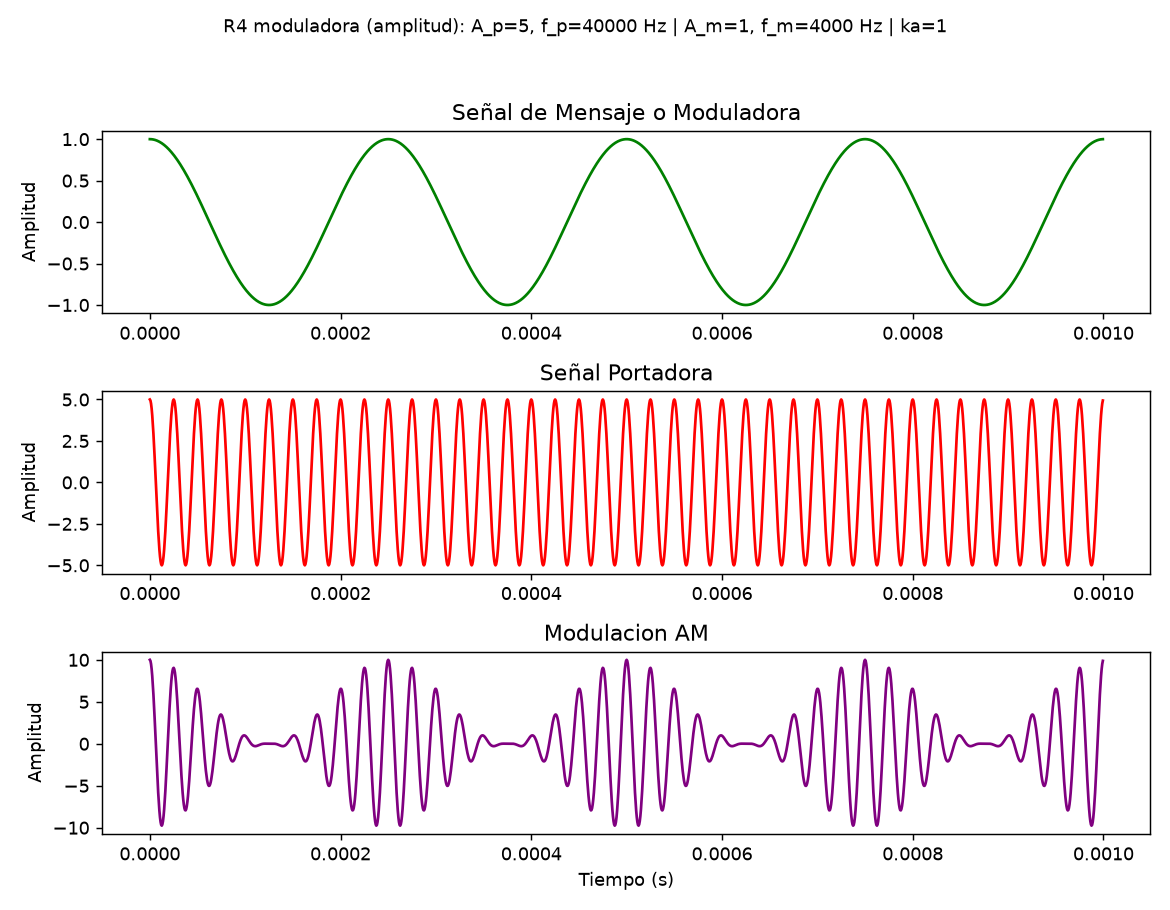
\includegraphics[width=0.75\linewidth]{imagenes/am-r4-moduladora-amplitud.png}
    \caption{Moduladora con menor amplitud: $A_m=1$}
\end{figure}

Este fue el resultado más llamativo de todas las pruebas: aunque la señal moduladora graficada aparte se ve mucho más chica, la señal AM final queda idéntica a la de la corrida base. Revisando la fórmula usada en el código, $A_m$ no aparece en ningún lado del cálculo de la modulación AM: solo se usa para graficar la moduladora como señal independiente. La profundidad de la modulación (cuánto \textit{se hunde} la envolvente) queda determinada únicamente por $k_a$, no por la amplitud real de la señal de mensaje.

Por último, subimos la frecuencia de la moduladora a 10000 Hz (achicando la ventana de tiempo para seguir viendo la misma cantidad de ciclos de envolvente):

\begin{figure}[h!]
    \centering
    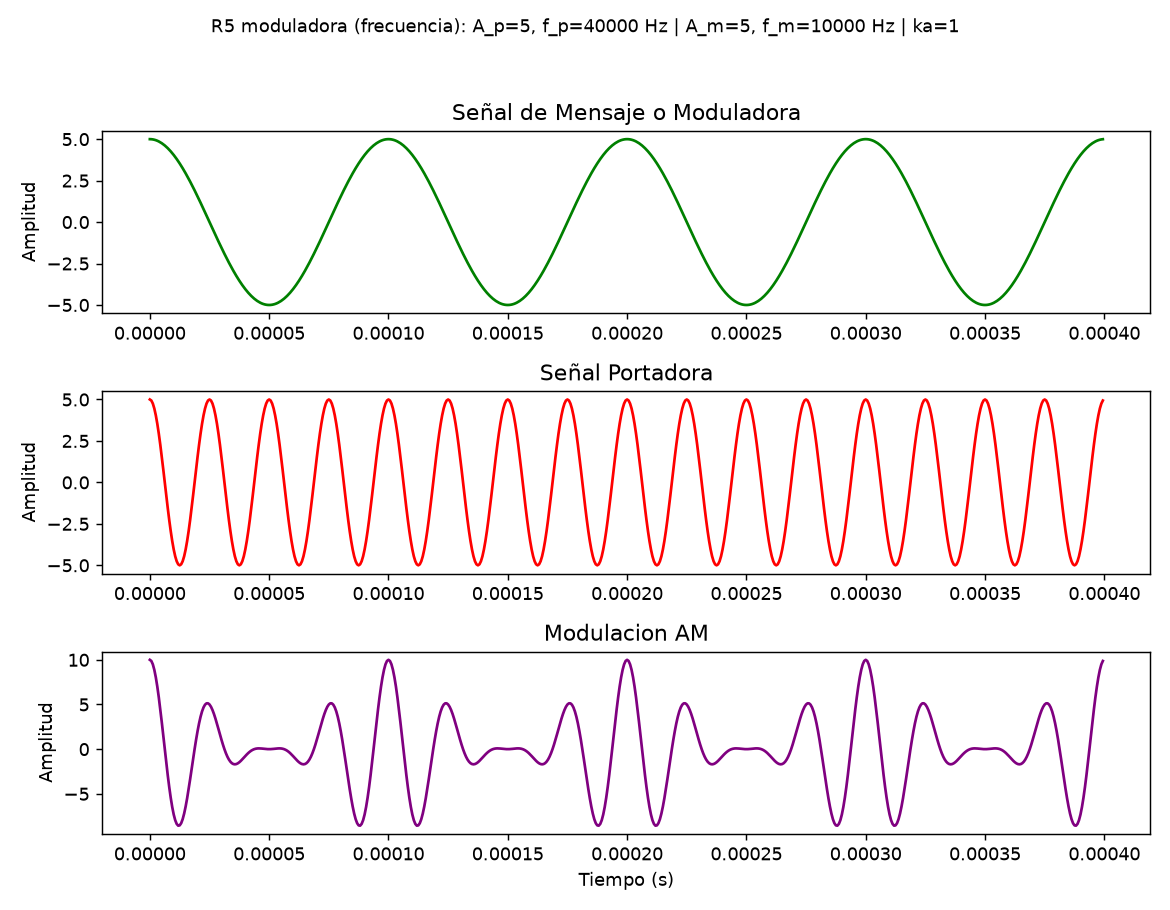
\includegraphics[width=0.75\linewidth]{imagenes/am-r5-moduladora-frecuencia.png}
    \caption{Moduladora con mayor frecuencia: $f_m=10000$ Hz}
\end{figure}

Al acercarse la frecuencia de la moduladora a la de la portadora, entran muchos menos ciclos de portadora dentro de cada lóbulo de la envolvente. Se nota que la envolvente ya no queda tan prolija: con pocos ciclos de portadora para dibujarla, se pierde la suavidad del contorno. Esto ilustra por qué en un sistema real la portadora tiene que ser bastante más rápida que la señal de mensaje: si no hay suficientes ciclos de portadora por cada variación de la moduladora, la envolvente deja de representarse con fidelidad.

\subsection*{Variando el índice de modulación}

Volviendo a los valores de la corrida base, probamos dos valores de $k_a$ distintos de 1. Con $k_a=0.3$ (submodulación):

\begin{figure}[h!]
    \centering
    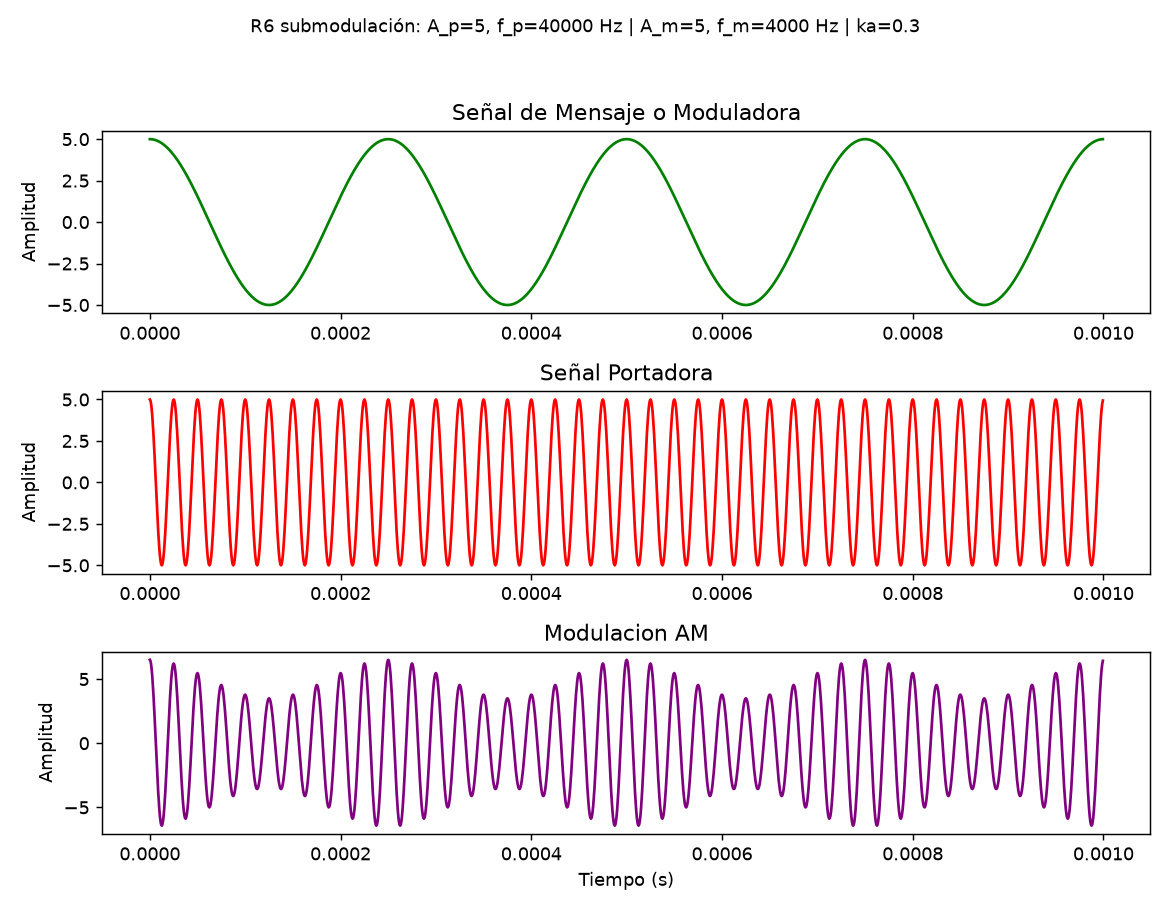
\includegraphics[width=0.75\linewidth]{imagenes/am-r6-submodulacion.png}
    \caption{Submodulación: $k_a=0.3$}
\end{figure}

La envolvente ya no llega a tocar el cero: se queda oscilando entre valores siempre positivos. Esto es la submodulación: se está usando menos rango dinámico del que la portadora podría aprovechar, lo que en un sistema real significa transmitir con menos eficiencia de la posible.

Con $k_a=2.5$ (sobremodulación):

\begin{figure}[h!]
    \centering
    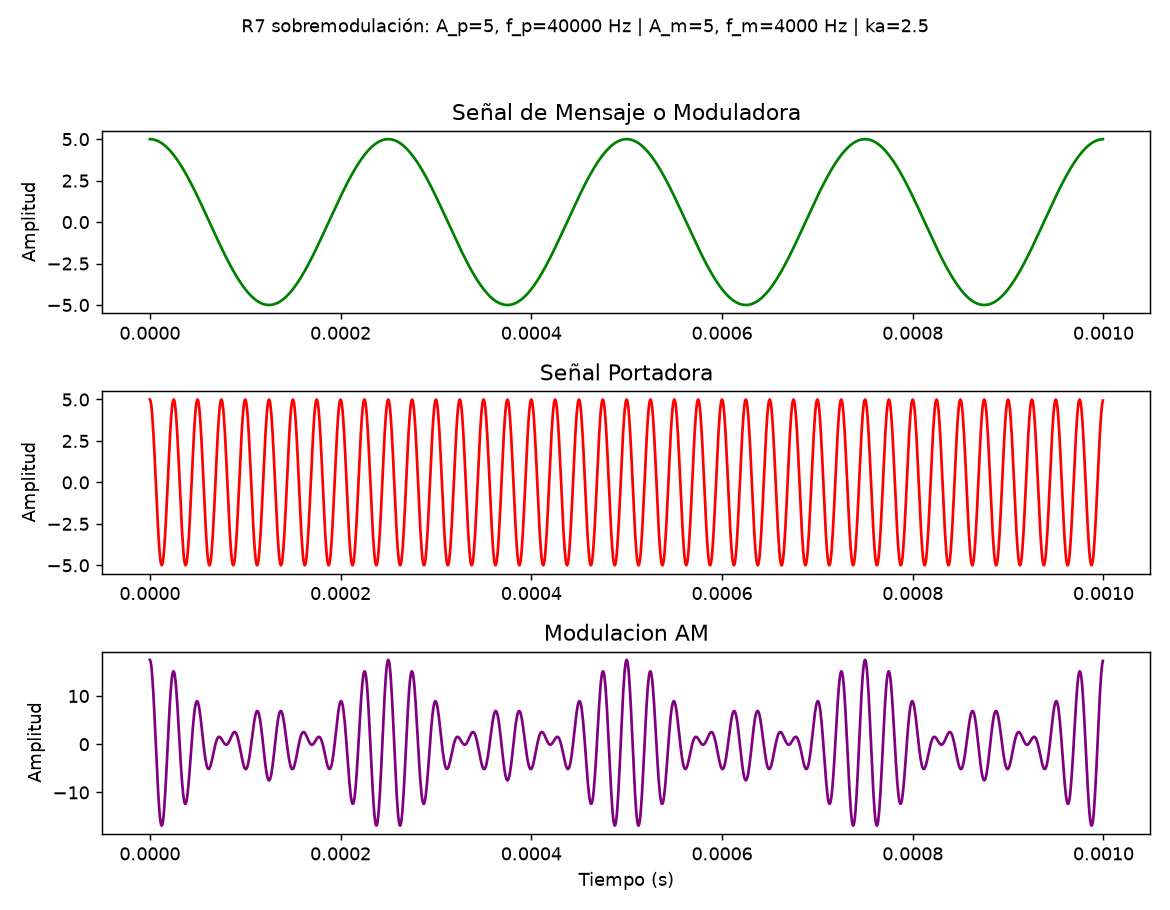
\includegraphics[width=0.75\linewidth]{imagenes/am-r7-sobremodulacion.png}
    \caption{Sobremodulación: $k_a=2.5$}
\end{figure}

Se ve claramente un rizado adicional cerca de los cruces por cero de la envolvente, que no estaba presente en la corrida base. Esa es la distorsión típica de la sobremodulación: al superar $k_a=1$, la envolvente se cruza consigo misma y ya no representa fielmente a la señal moduladora, lo que en la práctica generaría errores al recuperar la información en el receptor.

\subsection*{Conclusión}

Jugando con los parámetros del código pudimos separar el efecto de cada uno sobre la señal AM resultante. La amplitud de la portadora ($A_p$) solo escala el resultado sin cambiar su forma, y la frecuencia de la portadora ($f_p$) solo cambia cuántos ciclos de portadora entran por cada lóbulo de la envolvente, también sin afectar su forma. En cambio, la amplitud de la moduladora ($A_m$) no tiene ningún efecto sobre la señal AM en esta implementación: todo el peso de la modulación depende del índice $k_a$. La frecuencia de la moduladora ($f_m$), en cambio, sí es crítica: cuanto más se acerca a la frecuencia de la portadora, menos ciclos de portadora quedan disponibles para dibujar cada lóbulo de la envolvente, y la modulación se vuelve menos fiel. Finalmente, el índice de modulación resultó ser el parámetro más determinante de todos: valores menores a 1 dejan la envolvente sin llegar a cero (submodulación, poco eficiente), y valores mayores a 1 la distorsionan con rizado adicional (sobremodulación, poco fiel). En conjunto, estas pruebas muestran por qué en un sistema de comunicación real la relación entre $f_p$ y $f_m$, y el ajuste correcto de $k_a$, son decisiones de diseño tan importantes: determinan tanto la fidelidad como la eficiencia de la transmisión.

% ==================== BIBLIOGRAFÍA ====================
\seccionprincipal{Bibliografía}

Stallings, W. \textit{Comunicaciones y Redes de Computadoras}.

\end{document}
